\documentclass[tikz,border=2pt]{standalone}
\usepackage[T1]{fontenc}
\usepackage[utf8]{inputenc}
\usepackage{amsmath,amssymb}

% ACM
%\usepackage[tt=false, type1=true]{libertine}
%\usepackage[varqu]{zi4}
%\usepackage[libertine]{newtxmath}

% IEEE
\renewcommand{\sfdefault}{phv}
\renewcommand{\rmdefault}{ppl}
\renewcommand{\ttdefault}{pcr}
\usepackage{mathptmx}

\usepackage{pgfplots}
\pgfplotsset{compat=1.18}
\usepgfplotslibrary{groupplots}
\usepgfplotslibrary{colormaps}
\tikzset{
fill-color/.style={
	color of colormap={#1},
	draw=.!80!black,
	fill=.!80!white,
},
normal-color/.style={
	color of colormap={#1},
	draw=.,
},
mydashed/.style={dash pattern=on 6pt off 4pt}
}

\makeatletter
\pgfplotsset{
groupplot xlabel/.initial={},
every groupplot x label/.style={
	at={($({\pgfplots@group@name\space c1r\pgfplots@group@rows.west}|-{\pgfplots@group@name\space c1r\pgfplots@group@rows.outer south})!0.5!({\pgfplots@group@name\space c\pgfplots@group@columns r\pgfplots@group@rows.east}|-{\pgfplots@group@name\space c\pgfplots@group@columns r\pgfplots@group@rows.outer south})$)},
	yshift=.5ex,
	anchor=north,
},
groupplot ylabel/.initial={},
every groupplot y label/.style={
	rotate=90,
	at={($({\pgfplots@group@name\space c1r1.north}-|{\pgfplots@group@name\space c1r1.outer
			west})!0.5!({\pgfplots@group@name\space c1r\pgfplots@group@rows.south}-|{\pgfplots@group@name\space c1r\pgfplots@group@rows.outer west})$)},
	anchor=south
},
execute at end groupplot/.code={%
	\node [/pgfplots/every groupplot x label]
	{\pgfkeysvalueof{/pgfplots/groupplot xlabel}};  
	\node [/pgfplots/every groupplot y label] 
	{\pgfkeysvalueof{/pgfplots/groupplot ylabel}};  
}
}

\def\endpgfplots@environment@groupplot{%
\endpgfplots@environment@opt%
\pgfkeys{/pgfplots/execute at end groupplot}%
\endgroup%
}
\makeatother

% Code from Christian Feuersänger
% https://tex.stackexchange.com/questions/54794/using-a-pgfplots-style-legend-in-a-plain-old-tikzpicture#54834

% argument #1: any options
\newenvironment{customlegend}[1][]{%
\begingroup
% inits/clears the lists (which might be populated from previous
% axes):
\csname pgfplots@init@cleared@structures\endcsname
\pgfplotsset{#1}%
}{%
% draws the legend:
\csname pgfplots@createlegend\endcsname
\endgroup
}%

% makes \addlegendimage available (typically only available within an
% axis environment):
\def\addlegendimage{\csname pgfplots@addlegendimage\endcsname}


\begin{document}
% This file was created with tikzplotlib v0.10.1.
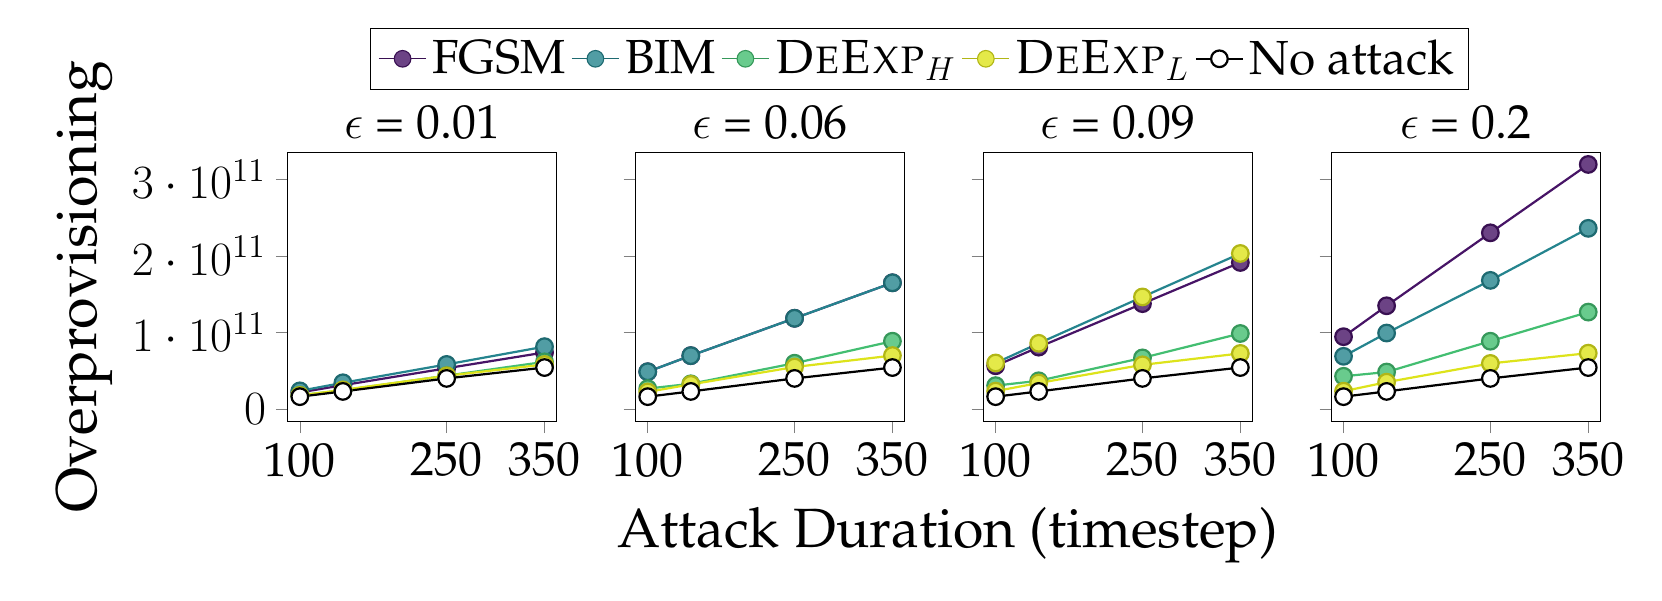
\begin{tikzpicture}
\definecolor{darkgray176}{RGB}{176,176,176}
\definecolor{green}{RGB}{0,128,0}
\definecolor{lightgray204}{RGB}{204,204,204}
\definecolor{purple}{RGB}{128,0,128}
\definecolor{yellow}{RGB}{255,255,0}

\begin{groupplot}[group style={group size=4 by 1},
width=5cm, height = 5cm,
xlabel style={font=\huge},
ylabel style={font=\huge},
xticklabel style={font=\LARGE},
yticklabel style={font=\LARGE},
title style={font=\LARGE,yshift=-1ex},
groupplot xlabel = {\fontsize{20}{33} \selectfont Attack Duration (timestep)},
xtick={100,250,350},
xticklabels={100,250,350},
yticklabel style={%
	scaled y ticks = false,
	/pgf/number format/.cd,
},
xticklabel style={%
	scaled y ticks = false,
	/pgf/number format/.cd,
	fixed,
	precision=0,
	fixed zerofill,
	1000 sep={\,},
},colormap/viridis
]
\nextgroupplot[
tick align=outside,
tick pos=left,
title={\(\displaystyle \epsilon\) = 0.01},
xmin=87.5, xmax=362.5,
ylabel={Overprovisioning},
ymin=-15966689306.3325, ymax=335301464252.682,
%ytick={-50000000000,0,50000000000,100000000000,150000000000,200000000000,250000000000,300000000000,350000000000},
%yticklabels={\ensuremath{-}0.5,0.0,0.5,1.0,1.5,2.0,2.5,3.0,3.5}
]
\addplot [thick, normal-color={50}, mark=*, mark size=3, mark options={solid,fill-color={50}}]
table {%
100 21810890000
144 31218450000
250 53329240000
350 73957700000
};
\addplot [thick, normal-color={450}, mark=*, mark size=3, mark options={solid,fill-color={450}}]
table {%
100 23849690000
144 34390840000
250 58358820000
350 81554280000
};
\addplot [thick, normal-color={700}, mark=*, mark size=3, mark options={solid,fill-color={700}}]
table {%
100 18136850000
144 24604180000
250 43675280000
350 61711420000
};
\addplot [thick, normal-color={950}, mark=*, mark size=3, mark options={solid,fill-color={950}}]
table {%
100 17900150000
144 25117590000
250 43549290000
350 58283120000
};
\addplot [thick, black, mark=*, mark size=3, mark options={solid, fill=white}]
table {%
100 16282590000
144 23109360000
250 40097050000
350 54285950000
};

\nextgroupplot[
scaled y ticks=manual:{}{\pgfmathparse{#1}},
tick align=outside,
tick pos=left,
title={\(\displaystyle \epsilon\) = 0.06},
xmin=87.5, xmax=362.5,
ymin=-15966689306.3325, ymax=335301464252.682,
yticklabels={}
]
\addplot [thick, normal-color={50}, mark=*, mark size=3, mark options={solid,fill-color={50}}]
table {%
100 48807690000
144 69813900000
250 118565880000
350 164882290000
};
\addplot [thick, normal-color={450}, mark=*, mark size=3, mark options={solid,fill-color={450}}]
table {%
100 48807690000
144 69813900000
250 118565880000
350 164882290000
};
\addplot [thick, normal-color={700}, mark=*, mark size=3, mark options={solid,fill-color={700}}]
table {%
100 26823430000
144 33078520000
250 59930750000
350 88649710000
};
\addplot [thick, normal-color={950}, mark=*, mark size=3, mark options={solid,fill-color={950}}]
table {%
100 22492540000
144 32304080000
250 54959400000
350 69929170000
};
\addplot [thick, black, mark=*, mark size=3, mark options={solid, fill=white}]
table {%
100 16282590000
144 23109360000
250 40097050000
350 54285950000
};

\nextgroupplot[
scaled y ticks=manual:{}{\pgfmathparse{#1}},
tick align=outside,
tick pos=left,
title={\(\displaystyle \epsilon\) = 0.09},
xmin=87.5, xmax=362.5,
ymin=-15966689306.3325, ymax=335301464252.682,
yticklabels={}
]
\addplot [thick, normal-color={50}, mark=*, mark size=3, mark options={solid,fill-color={50}}]
table {%
100 56595540000
144 80922720000
250 137664080000
350 191418570000
};
\addplot [thick, normal-color={450}, mark=*, mark size=3, mark options={solid,fill-color={950}}]
table {%
100 60222480000
144 85907990000
250 146414470000
350 203130440000
};
\addplot [thick, normal-color={700}, mark=*, mark size=3, mark options={solid,fill-color={700}}]
table {%
100 30705710000
144 37004500000
250 66858550000
350 98710010000
};
\addplot [thick, normal-color={950}, mark=*, mark size=3, mark options={solid,fill-color={950}}]
table {%
100 23529680000
144 34106770000
250 57813990000
350 72699850000
};
\addplot [thick, black, mark=*, mark size=3, mark options={solid, fill=white}]
table {%
100 16282590000
144 23109360000
250 40097050000
350 54285950000
};

\nextgroupplot[
scaled y ticks=manual:{}{\pgfmathparse{#1}},
tick align=outside,
tick pos=left,
title={\(\displaystyle \epsilon\) = 0.2},
xmin=87.5, xmax=362.5,
ymin=-15966689306.3325, ymax=335301464252.682,
yticklabels={}
]
\addplot [thick, normal-color={50}, mark=*, mark size=3, mark options={solid,fill-color={50}}]
table {%
100 94515190000
144 134861470000
250 230068630000
350 319334730000
};
\addplot [thick, normal-color={450}, mark=*, mark size=3, mark options={solid,fill-color={450}}]
table {%
100 68957290000
144 99308070000
250 168026760000
350 235940380000
};
\addplot [thick, normal-color={700}, mark=*, mark size=3, mark options={solid,fill-color={700}}]
table {%
100 42875160000
144 48434720000
250 88643840000
350 126626020000
};
\addplot [thick, normal-color={950}, mark=*, mark size=3, mark options={solid,fill-color={950}}]
table {%
100 23389490000
144 35207260000
250 59628210000
350 73054670000
};
\addplot [thick, black, mark=*, mark size=3, mark options={solid, fill=white}]
table {%
100 16282590000
144 23109360000
250 40097050000
350 54285950000
};
\end{groupplot}
\begin{customlegend}[colormap/viridis,
legend entries={ % <= in the following there are the entries
FGSM,
BIM,
\textsc{DeExp}$_H$,
\textsc{DeExp}$_L$,
No attack,
},
legend columns=-1,
legend style={at={(15,5)},font=\LARGE}] % <= to define position and font legend
% the following are the "images" and numbers in the legend
\addlegendimage{fill-color={50}, mark=*, mark size=3, mark options={solid}}
\addlegendimage{fill-color={450}, mark=*, mark size=3, mark options={solid}}
\addlegendimage{fill-color={700}, mark=*, mark size=3, mark options={solid}}
\addlegendimage{fill-color={950}, mark=*, mark size=3, mark options={solid}}
\addlegendimage{thick,fill=white, draw=black, mark=*, mark size=3, mark options={solid}}
\end{customlegend}
\end{tikzpicture}
\end{document}
